
%
%  $Description: Author guidelines and sample document in LaTeX 2.09$ 
%
%  $Author: ienne $
%  $Date: 1995/09/15 15:20:59 $
%  $Revision: 1.4 $
%

\documentclass[times, 10pt,twocolumn]{article} 
\usepackage{latex8}
\usepackage{times}
\usepackage{graphicx}
\usepackage[font={it}]{caption}
\graphicspath{{Users/pedrolopes/Documents/PADI1314}}

%\documentstyle[times,art10,twocolumn,latex8]{article}

%------------------------------------------------------------------------- 
% take the % away on next line to produce the final camera-ready version 
\pagestyle{empty}

%------------------------------------------------------------------------- 
\begin{document}

\title{PADI-DSTM}



\maketitle
\thispagestyle{empty}


%------------------------------------------------------------------------- 
\Section{Introduction}
Since the beginning of the computer revolution in the world, the distributed systems have played a major role in the technologies' innovation and development. This area comprises a great set of different technologies and applications, like network applications, telecommunication networks, parallel computation, etc. In recent years we have been witnessing a new era in technology, the Cloud era. Today the Cloud is the new "big thing" in computers and mobile devices, everyone can access everything  everywhere! As such, the transactional shared memory systems are increasingly important in the world of technology, because nowadays the computers and mobile devices are using the cloud storage, and capacities, not only for save data but also for run programs, like the Amazon Silk, that is a web browser that processes the requests from the clients in the Amazon servers, and the client's devices only have to renderer the result data, to present the result. Due to this evolution of the distributed systems, the PADI-DSTM appeared.This library intends to implement a distributed system to manage objects stored in a distributed shared memory, that are shared by transactional applications that are being executed in different machines. This library intends to provide an easy way for the programmers doesn't have to deal with the distributed systems and transactions problems, like deadlocks, inconsistent data or data that disappears because a server fails, etc. The programmers only have to integrate the PADI-DSTM in his application, and the management of the transactional shared memory is all made by the library.

%------------------------------------------------------------------------- 
\Section{Architecture Overview}

This work focuses on implementing a transactional shared memory system, which stores variables of PADInt type. These variables will be shared between the multiple clients of the system and will be located in a set of transactional servers, that replicate information in case of failure occurrence. Clients, recurring to the PADI-DSTM library, create and access variables on the system recurring to a master server, which maintains information about storage servers, and manages the location of each PADInt. Once accessed, clients can execute transactions, that encapsulate read and write operations on a subset of these variables, preserving the Atomicity, Consistency, Isolation and Durability (ACID) properties. One of the main concerns of this work is trying to implement the system in a decentralized way, minimizing the interaction with centralized entities. For doing so, it considers two roles for the transactional servers. They can act as participants or as the transaction coordinator, in contrast with the approach of giving the coordination role to the master server, which would impact decentralization. The interactions with the master server will be only for creating and accessing data objects. The system will consider a fault model which tolerates one silent failure. For doing so, it implements an active replication protocol with 3 replicas. The system will follow a two-phase commit protocol for executing the transactions, which, as mentioned before, will take as coordinator the transactional server, and as participants the servers which hold the involved data objects. Finally, the master server will be able to mediate the load between transactional servers, reallocating resources in order to preserve the equal distribution of network and storage loads, which favors the system's scalability. The next sections will expose the system's behavior with more detail.

%------------------------------------------------------------------------- 
\SubSection{Data Structures}

Our PADI-DSTM library contains multiple types of data structures in the different components of the system, each component has it's own structures, with different goals, and the main structure is the PADInt, which is used by the different components.

First of all the Master server, it contains a few structures: the list of the servers that are active, which is constantly being updated (servers send heartbeat messages to the master), so that the master can refresh the servers list, and that list will be used for the load balancing algorithm, which will be explained later. The master also contains a table with the servers' locations of each PADInt, so that when the clients contacts the master by the AcessPADInt method, the master only have to access the table with the PADInt uid, and give the server's URL to the client, and he contacts the servers to get a remote reference to the object. When a client makes a CreatePADInt request to the master, it only has to generate, with the load balancing algorithm, the 3 servers in which the PADInt will be stored, and add the pair (uid, servers) to the table of locations. The master is also the one who generates the timestamps and IDs for the transactions, so when a client wants to make a transaction he has to request the "transaction's context" to the master; in this case, the client receives a transaction ID, timestamp, and, when he commits, the client also has to request the URL of coordinator for the 2PC protocol, which is a server chosen by the master. For having a log of the transactions the master also stores the transactions' ids that have started, and having finished, this implies that if one transaction id only exists in the list of started transactions, this means that the transaction has been aborted or is in course.

\begin{figure}[h!]

\centering

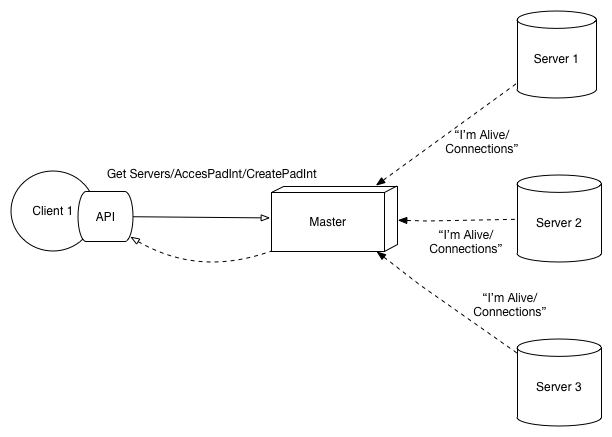
\includegraphics[scale=0.4]{Client-Master.png}

\caption{Client's requests to master and servers' heartbeat messages}

\end{figure}

The PADInt object is the main one in our architecture, it is stored in the transactional servers, and each PADInt exists in three servers, in order to tolerate faults. Each of the three objects is always updated to the last version, because when the changes to the object are committed, the new values are propagated to the other servers in which the object is stored. The PADInt object contains different sub-objects, its UID (to make each PADInt unique), its value, an array of the servers in which it is stored (we decided that each object knows its own location). The PADInt object also contains a timestamp that it is used to control the access to the variable in memory; in this case, if the client timestamp is lower than the timestamp of the object it means that the client has an old version of the object and the transaction is aborted. The PADInt also contains a list of temporary values, that are being modified by the clients, that are according to the transaction ID. When the library receives the remote object from the master, from a CreatePADInt or an AccessPADInt request made by the client, the library creates a new structure that in fact is a local copy of the PADInt, in which it stores the three remote references, for the "real PADInt" in the transactional servers, and returns that local copy to the client. In fact, the client is modifying the copy and not the remote object, so when he makes a commit request, the servers access its own PADInts involved in the transaction and transfers the values from the temporary list to the real value of the PADInt, and stores the old value in case of rollback if the transaction fails.

The transactional servers' main structures are the list of PADInts and the pending requests: this list is the one where are stored the requests made to the server; if the server is in a Freeze state, when it recovers, it iterates over the list runs every request that was made previously.

\begin{figure}[h!]

\centering

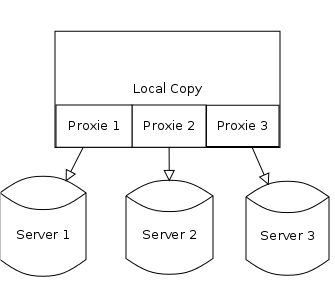
\includegraphics[scale=0.4]{Padint.png}

\caption{PADInt's local copy structure}

\end{figure}

\SubSection{Load Balancing}

The balancing of the system is always made in the creation of PADInts: when the master receives a CreatePADInt request, it calls the function for selecting the servers with the lower load. That function calculates the number of PADInts that are stored in each server, with the information of the active servers and the PADInts locations that are stored in the Master server. This function always chooses the 3 servers that currently store the least amount of PADInts, and it's always executed when a new creation request arrives, so the balancing is always assured, because all the servers should have similar number of objects. This implicitly leads to another advantag:, the number of connections is balanced too, since the servers that are the ones with less load, and theoretically with less number of connections.

After the balancing, the servers that were chosen are returned to the PADI-DSTM library, that will create a connection to servers and request the creation for the PADInt.

%------------------------------------------------------------------------- 
\SubSection{Responsibilities}

As seen before, our approach will be divided in three components: a master, a set of transactional servers and a client, each one of them with distinct roles.
The master has two main responsibilities: the first one is to store meta-data regarding transactional servers and data objects existing in PADI-DSTM. It stores, among other information, objects' locations and uid, or transactional servers' locations and network load. The second role of master server is to mediate the creation and access to shared variables. Clients connect to the master for getting remote objects that represent variables. In case of creation, the master will choose the least loaded transactional servers and execute a create operation. This approach contrasts with the implementation of a periodical load balancing algorithm for re-allocating all the data objects in the entire system. This paper opts for the first one for being the most efficient one, avoiding freezing the entire system for balancing the network load.
The second one, the transactional servers, will store and execute the changes made to the data objects, acting as participants of a distributed transaction protocol. They are responsible for managing the variable locks and committing or aborting transactions depending on the conditions they have for maintaining the ACID properties of each transaction. They also inform the master of their activity through a heartbeat message, informing the master they are still operating. Transactional servers will also act as coordinators for the transactions triggered by the clients. Clients connect to the servers that are currently storing the variables they want to modify and trigger a two-phase commit protocol on the coordinating transactional server, once they have ended the modifications of every used variable.
Finally, clients will execute the calls that use the PADI-DSTM library, invoking the creation/access to the objects on the master and manipulating them on the transactional servers.

\begin{figure}[h!]
	\centering
	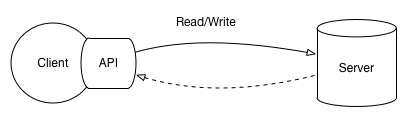
\includegraphics[scale=0.45]{Client-Server.png}
	\caption{Client-Server connections}
\end{figure}

%------------------------------------------------------------------------ 
\SubSection{Concurrency Control}

With a distributed system, there's a problem that is inherent to this type of architecture: concurrent access to shared objects. In this particular case, we have to take into consideration that objects can be accessed by multiple clients and, when committing the changes, the objects may be accessed by several servers as well.
To manage this type of concurrency, we will be using timestamp-based concurrency control. This type of approach assigns a timestamp (which can be a time value or a sequence number) to the transactions that want to have access over a certain object. This object also keeps a timestamp of its own and also keeps track of the latest transaction that read/wrote the object's value. With this kind of approach, the transactions are forced, in a sense, to access the object in a specific order, so that there are no actual parallel accesses.
One aspect that is important to mention is that there is still a lock on the object that is being accessed, though this is not a "fully grown" lock as it would be in database lock-based concurrency control. The lock is to prevent concurrent access to an object, though the time the lock is locked is significantly smaller and there is no chance of deadlocking since it is immediately released when it's no longer needed, as opposed to lock-based concurrency control in which the locks are released at the end of the transaction.

%------------------------------------------------------------------------- 
\SubSection{Transactional Algorithms}

For guaranteeing the conformity with ACID properties, our solution will implement a transaction protocol between the servers involved in an operation. It implements a slight variation of a Two-phase commit protocol (2PC), where a given transactional server plays the role of coordinator, and the transactional servers that are storing the PADInts act as participants. Taking one of the transactional server machines as the transaction coordinator, it is possible since we can assume that (i) taking a random transactional server to coordinate the transaction favors system decentralization, (ii) clients should not act as coordinators since they must be the least logically capable machines. This way, our solution avoids the bottleneck of centralizing the coordination on the master server. On the other hand, the coordination task being given to another unrelated transactional server, it can lead to protocol deadlocks, since it is assumed transactional servers can crash.
The protocol initiates calling beginTx() operation, which gets information about the transaction coordinator from the master server, through the PADI-DSTM library. This object has an endpoint with a given address, and creates a transaction identifier (tid). Each operation executed on each of transactional server will carry the transaction id and address of coordination endpoint so that they join the current transaction. Once all servers are joined, the protocol carries out through the following two phases.

\begin{itemize}

\item[--] Phase one: Voting

\begin{enumerate}
	
\item The coordinator sends a \emph{prepare} message to each participant.

\item Based on the operation's viability, each participant replies \emph{yes} or \emph{no} to the prepare request. In affirmative case, it prepares to commit saved objects into persistent storage. In case of a negative answer, it has to completely abort the transaction.

\end{enumerate}

\item[--] Phase two: Deciding

\begin{enumerate}

\item The coordinator decides whether the transaction commits or aborts based on the votes returned from the participants. If all the participants vote to commit, and no failure has occurred, the coordinator decides to commit the transaction and sends a \emph{doCommit} request to every participant. In case any of the participants vote to abort, the coordinator signals all of them to abort the transaction.

\item The participants receive a response from coordinator and do whatever it prescribes them to do (commit or abort). In case of a \emph{doCommit}, the participant returns a \emph{haveCommited} call to inform the coordinator that the transaction is finished. In case of abort, they simply abort the transaction.

\end{enumerate}

\end{itemize}

Once its assumed that transactional servers can crash and the network can delay the delivery of messages, the protocol peers (coordinator and participants) are required to limit the time they wait for a response. Therefore, the protocol implements a series of timeout procedures in order to avoid situations where the peers wait indefinitely. 
Firstly, consider the situation where the participant voted \emph{yes} and is waiting for a decision from the coordinator. Since this is assumed as not crashing, the only reason the participant can wait a long period of time is due to a network delay. For resolving this issue, the participant, in presence of a similar situation, must inquiry the coordinator for a decision (through a \emph{getDecision} call). The coordinator then replies and the participant gets its decision.
The second situation related to the phase where the coordinator waits for the votes from all the participants: if one or more of these servers crash or has a network delay, the coordinator must not wait indefinitely. In this case, it starts a timer. Once it reaches timeout, the coordinator sends \emph{doAbort} messages to all the transaction participants.

\begin{figure}[h!]
	\centering
	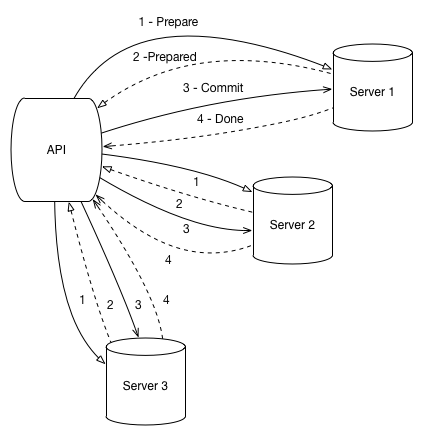
\includegraphics[scale=0.45]{2PC.png}
	\caption{Our Two-phase Commit Protocol approach}
\end{figure}

%------------------------------------------------------------------------- 
\SubSection{Distributed Protocols}

As indicated above, our approach will take into account the problem of overloading servers, in this case, the problem is that, at a certain point in time, it is possible that some servers will have greater load than others, or, if new servers connect to the master, those servers will be empty, and the others can be full, and because they have all the objects, the requests will be always made to the loaded servers, while the new ones remain empty. To solve the problem our solution will be divided in two parts: the first part is that the master will have a registry of the objects' locations, so the master can always see which servers have greater load; in the second part of the solution, the master, as mentioned above, will receive heartbeat messages, which will alert the master of which servers are still active. With that information, the master will update his registry of the active servers, and when a new client requests the server some object, the master will give him the less loaded server. 

Regarding the replication aspect of our solution, we have an active replication protocol. This protocol is applied during the creation of a PADInt and, when a transaction commits successfully, the process of updating the PADInt's replicas, to keep the data consistency.
When a client creates a PADInt, the master returns to the PADI-DSTM three servers (with the least amount of PADInts), where the PADInt will be stored (further explanation of the algorithm is addressed in the sub-section "Load Balancing"). For the update part, since the PADInt holds a list of its replicas, when a transaction commits, the replicas are updated right after the "original" PADInt, thus keeping the data consistent.
This type of replication allows us to easily access and alter a client-side local copy since it has a list of all its replicas' locations. This way, we can easily send the "final" value (ie, the last value written to the PADInt before a successful commit) to the replicas and, when \emph{TxCommit()} is called, we have two possible outcomes: if the transaction commits successfully, the "original" PADInt passes its final value to the copies and that value is persisted in all of them; if the transaction has to abort, all PADInt replicas and the "original" one rollback, which basically sets the \emph{value} field equal to the \emph{oldValue} field, initialized with the PADInt's original value when the transaction begins.

%------------------------------------------------------------------------- 
\SubSection{Deadlock Detection and Abort Recovery}

Bearing in mind that we're using timestamps to prevent concurrent access to shared objects, the greatest advantage when using this type of concurrency control is that there are no deadlock situations, since the access to shared objects aren't locked by another data type, like the locks used in database transactions or the OS's mutexes.
Even though this concurrency control method avoids deadlock through its implementation, there are some situations where the occurring transactions abort without a conflict of two (or more) of those transactions accessing the same shared object. This sort of thing happens when, for example, a transaction T1 has a timestamp value of 100 and another transaction T2 has a timestamp value of 200. If T2 tries to read an object (without altering its value) before T1, though there are no read-write/write-write/write-read conflicts, both T1 and T2 must abort because the access to the object wasn't sequential (since T1 has a lower timestamp value than T2).
To overcome what was stated above, we will take into account what actions the transactions want to execute. By doing so, if two transaction only read the value from an object without altering it, even if they perform these actions inconsistently with the assigned timestamps, there is no need to abort because the operations' outcome will never generate an inconsistency, as long as there aren't any modifications to the object's value.

Since our concurrency control was based on timestamps (one assigned to the PADInt and another to the client accessing it) without any actual mechanism of locking (only a boolean: true, if the PADInt can't be accessed; false otherwise), there is no risk of deadlocking. Due to the optimistic concurrency control system we adopted, the "lock" is released as soon as the actions performed on the PADInt are executed.
With our type of approach, a transaction may had to abort only because a client that had a higher timestamp only read a PADInt's value before another client with a lower timestamp. This doesn't happen because all of the reading operations over a PADInt occur in the client's local copy. So, in the end, the operations that may actually affect a transaction's performance are the writing operations. And, with that, the problem of aborting a transaction or a cascading abort operation are directly related to the access sequence of the clients' writing operations.

\Section{Conclusions}

In this article we present a solution for PADI-DSTM. With the adopted approaches to the problem we believe that our solution will not have much problems in terms of scalability, because connect new servers to master is very easy to be done, the load balance solution will try to ensure the load equality between servers. Our load balance solution helps to control the number of connections clients-servers, because the master is the one who controls which servers the client receives to try to bind.

Our solution gives particular emphasis to the Two-phase commit protocol to control the ACID problems of transactions, and because our transaction coordinator is the client, the master it isn't a bottleneck in the system. Other solutions could be adopted, like servers communicate between each other in the commit phase to store the data, this could make our transactions faster, because the 2PC protocol is a slow algorithm, but this solution will bring us other sort of problems, like the main server fail during the commit phase.

Finally, we believe that our solution can be improved, and we expect to do so in the near future.

%------------------------------------------------------------------------- 

\bibliographystyle{latex8}
\bibliography{latex8}

\begin{thebibliography}{9}
 
\bibitem{Distributed Systems, Concepts and Design}
George Coulouris, Jean Dollimore, Tim Kindberg, Gordon Blair,
   Distributed Systems, Concepts and Design, 
   Pearson,
   5th edition,
   2012.

\end{thebibliography}

\end{document}
